\documentclass[10dd, a5paper]{article}

\usepackage[utf8x]{inputenc}
\usepackage[russian]{babel}

\usepackage{xcolor}
\definecolor{kvant-paper}{RGB}{238,213,172}
\pagecolor{kvant-paper}

\usepackage{graphicx}
\graphicspath{{./}}

\usepackage{fontspec}
\setmainfont[
Extension = .ttf,
BoldFont = SchoolBook Bold Cyrillic,
ItalicFont = SchoolBook Italic Cyrillic]{SchoolBook Cyrillic}
\usepackage{multicol}

\usepackage[labelsep=none, labelfont=it, font=footnotesize, singlelinecheck=false]{caption}
\captionsetup[table]{justification = raggedleft, skip=0pt}
\captionsetup[figure]{justification=raggedright}
\setcounter{figure}{3}

\usepackage[a5paper,hmargin=0.2cm, tmargin=0.1cm, bmargin=0.85cm, footskip=0.8cm]{geometry}

\newtheorem{exmp}{Пример}
\renewcommand{\exmp}{П\,р\,и\,м\,е\,р\quad\arabic{exmp}.\itshape}
\setcounter{exmp}{3}

\newtheorem{sol}{Решение}
\renewcommand{\sol}{Р\,е\,ш\,е\,н\,и\,е.\upshape}

\newtheorem{theor}{Теорема}
\renewcommand{\theor}{Т\,е\,о\,р\,е\,м\,а.\itshape}

\usepackage{amsmath}

\usepackage{sectsty}
\sectionfont{\fontsize{10dd}{8}\selectfont}

\usepackage{fancyhdr}

\usepackage{fancyhdr}
\usepackage{lipsum}
\newenvironment{Biglogo}
  {\par\medskip\noindent\minipage{\linewidth}}
  {\endminipage\par\vspace{1.5cm}}

\usepackage{tabularx}
\title{Преамбулка к Лабораторной работе - 6}
\author{Дмитрий Х.}

\begin{document}
\maketitle
Задачу выполнил. <<Квант>> сваял. Сделал все на \verb|\begin{minipage}|. Код страшный вышел. Вот так вот-с!
\newpage
\documentclass[10dd, a5paper]{article}

\usepackage[utf8x]{inputenc}
\usepackage[russian]{babel}

\usepackage{xcolor}
\definecolor{kvant-paper}{RGB}{238,213,172}
\pagecolor{kvant-paper}


\usepackage{graphicx}
\graphicspath{{./}}

\usepackage{fontspec}
\setmainfont[
Extension = .ttf,
BoldFont = SchoolBook Bold Cyrillic,
ItalicFont = SchoolBook Italic Cyrillic]{SchoolBook Cyrillic}
\usepackage{multicol}

\usepackage[labelsep=none, labelfont=it, font=footnotesize, singlelinecheck=false]{caption}
\captionsetup[table]{justification = raggedleft, skip=0pt}
\captionsetup[figure]{justification=raggedright}
\setcounter{figure}{3}

\usepackage[a5paper,hmargin=0.2cm, tmargin=0.1cm, bmargin=0.85cm, footskip=0.8cm]{geometry}

\newtheorem{exmp}{Пример}
\renewcommand{\exmp}{П\,р\,и\,м\,е\,р\quad\arabic{exmp}.\itshape}
\setcounter{exmp}{3}

\newtheorem{sol}{Решение}
\renewcommand{\sol}{Р\,е\,ш\,е\,н\,и\,е.\upshape}

\newtheorem{theor}{Теорема}
\renewcommand{\theor}{Т\,е\,о\,р\,е\,м\,а.\itshape}

\usepackage{amsmath}

\usepackage{sectsty}
\sectionfont{\fontsize{10dd}{8}\selectfont}

\usepackage{fancyhdr}

\setcounter{page}{52}

\begin{document}
\pagestyle{fancy}
\fancyfoot{}
\fancyfoot[LO]{\textbf{\LARGE\thepage}}
\setlength{\textfloatsep}{3dd}
\setlength{\belowdisplayskip}{1dd} \setlength{\belowdisplayshortskip}{1dd}
\setlength{\abovedisplayskip}{1dd} \setlength{\abovedisplayshortskip}{1dd}
\setlength{\parskip}{2dd}
%Figures row
\begin{figure}
\centering
\begin{minipage}{0.48\textwidth}
	\raggedleft
	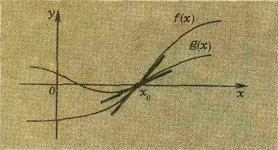
\includegraphics[width =\linewidth, height = 3.6cm]{fig1}
	\caption{.}
	\label{fig:left}
\end{minipage}%
\hspace{0.5cm}%
\begin{minipage}{0.48\textwidth}
	\raggedleft
	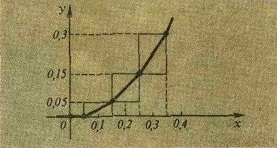
\includegraphics[width =\linewidth, height = 3.6cm]{fig2}
	\caption{}
	\label{fig:right}
\end{minipage}
\end{figure}
\setlength{\textfloatsep}{2dd}
\begin{multicols}{2}
\linespread{0.65}\selectfont
\noindent $f(x)/g(x)$ при значения $x$, приближающихся к $x_0$, если в этой точке числитель и знаменатель обращаются в нуль. Считаем $f(x)$ и $g(x)$ линейными вблизи точки $x_0$, малые кусочки их графиков заменяем касательными к к графикам этих функций в точке $x_0$. Таким образом, считаем, что\[f(x) = f'(x_0)(x-x_0), g(x)=g'(x_0)(x-x_0).\] Тогда, если $g'(x_0)\neq0$, то\[\frac{f(x)}{g(x)}=\frac{f'(x_0)(x-x_0)}{g'(x_0)(x-x_0)}=\frac{f'(x_0)}{g'(x_0)}.\] Надо понмить, что фактически это равеноство приближенное, но тем более точное, чем ближе $x$ к $x_0$. Мы получили правило, известное в математике как \itshape правило Лопиталя для раскрытия неопределенности типа $0/0$\upshape.

\linespread{0.65}\selectfont
{\footnotesize На языке пределов это правило читается так: предел отношения $\frac{f(x)}{g(x)}$ при $x\rightarrow x_0$, если $f(x_0)~=~0$ и $g(x_0)~=~0$, равен отношению производных $f'(x_0)$ и $g'(x_0)$:
{\setlength{\belowdisplayskip}{1dd} \setlength{\belowdisplayshortskip}{1dd}
\setlength{\abovedisplayskip}{1dd} \setlength{\abovedisplayshortskip}{1dd}
\[\begin{array}{cr}
\lim\limits_{x \to x_0} \frac{f(x)}{g(x)}=
\frac{f'(x_0)}{g'(x_0)}&(g'(x_0\neq 0)
\end{array}\]}}
\begin{exmp}
Составить таблицу значений функции \[f(x) = \frac{2x^2-x-
\sin\pi x/2}{\sqrt{x}-\cos(1-x)}\]вблизи точки $x=1$.
\end{exmp}
\begin{sol}
Результаты вычислений на МК В3-34 показаны в таблице 1. Применим правило Лопиталя
\begin{multline*}
(2x^2-x-\sin\frac{\pi}{2}x)'\vert_{x=1}=\\
= (4x-1-\frac{\pi}{2}\cos\frac{\pi}{2}x)\vert_{x=1} = 4 -1 =3,\\
(\sqrt{x}-\cos(1-x))'\vert_{x=1}=
\end{multline*}
\[=(\frac{1}{2\sqrt{x}}-\sin(1-x))\vert_{x=1}=\frac{1}{2}.\]
Следовательно, при стремлении $x$ к $1$ значения $f(x)$ приближаются к числу $3:(1/2)=6$. ИЗ таблицы видно, что ошибки в вычислениях начинаются довольно далеко от предела точности МК - уже при $x=1,0001$.
\end{sol}
\section*{Признак возрастания (убывания) функции на интервале}
\begin{theor}
Если в каждой точке интервала уголовой коэффициент (производная) к графику функция возрастает на этом интервале, а если меньше нуля - то убывает.
\end{theor}
\linespread{0.65}\selectfont
{\footnotesize Действительно, пусть угловой коэффициент касательной к графику функции больше нуля. Тогда касательная в лобой точке графика является поднимающейся прямой и, следовательно, лбой достаточно малый участок графика есть поднимающаяся линия. Интуитивно ясно, что график в целов есть поднимающаяся линия и, следовательно, функция возрастает. Аналогично, отрицательность производной во всех точках интервала влечет убывание функции на этом интервале.}
\linespread{0.8}\selectfont
\section*{Численное решение\\ дифференциальных уравнений}
Во многих случаях удается получить зависимость между велчинами, содержащую их производные, т.е. в виде \textit{дифференциального уравнения}. Далеко не всегда уравнение удается разрешить, т.е. найти функции, являющиеся решением данного дифферен-
\end{multicols}
\centering
\setlength{\textfloatsep}{2dd}
\begin{table}[b]
\caption{}
\small
\begin{tabular*}{\textwidth}{l@{\extracolsep{\fill}}|l|l|l|l|l|l}
$x$ & 1,1 & 1,01 & 1,001 & 1,0001 & 1,00001 & 1,000001\\
\hline
$f(x)$ & 6,1762693 & 6,0196529& 6.0039984 & 6,012024 & 6,1224489 & 7,5
\end{tabular*}
\end{table}
\end{document}

\newpage

\pagestyle{fancy}
\fancyhf{}
\renewcommand{\headrulewidth}{0pt}
\fancyfoot[RO]{\textbf{\LARGE\thepage}}
\noindent

\begin{minipage}[t][][t]{0.45\linewidth}
\begin{Biglogo}
\raggedright

\includegraphics[width=0.7\linewidth]{Kvant_logo}

\smallskip
\fontsize{9dd}{7dd}\selectfont
\raggedright
\textit{Основан в 1970 году}
\end{Biglogo}
\fontsize{8dd}{7dd}\selectfont
\raggedright
\itshape Научно-популярный физико-математический\\ журнал Академии наук СССР и Академии педагогических\\ наук СССР

\vspace{0.3cm}
\begin{minipage}[l]{0.1\linewidth}

\includegraphics[width=\linewidth]{nauka}
\end{minipage}%
\hspace{3dd}%
\begin{minipage}[с]{0.87\linewidth}
\fontsize{8dd}{6dd}\selectfont
\raggedright
Издательство <<Наука>>. Главная редакция физико-\\математической литературы
\end{minipage}
\end{minipage}%
\begin{minipage}[t][][b]{0.55\linewidth}

{\fontfamily{lmss}\fontsize{20dd}{6dd}\selectfont
\hspace{20dd}1988

{\fontsize{30dd}{6dd}\selectfont 4}
}
\vspace{1cm}

%Стилизуем содержаниее
\fontsize{17dd}{6dd}\selectfont{В номере:}

\fontsize{7dd}{6dd}\selectfont
\begin{tabularx}{\linewidth}{lX}
{\bf 2} & {\itshape И. Д. Новиков.} Вселенная как тепловая машина\\
{\bf 9} & {\itshape Ю. М. Львов, Л. А. Фейгн.} Ленгмюровские пленки --- путь к молекулярной электронике?\\
{\bf 14} & {\itshape М. Гарднер.} Рамсеевская теория графов\\
{\bf 21} & {\itshape} Интервью с американским математиком Рональдом Грэхемом\\
& \vspace{1dd}{\bf Задачник <<Кванта>>}\\
{\bf 27} & Задачи М1096-М1100, Ф110--Ф1112\\
{\bf 28} & Problems М109--М1100, Ф1108-Ф1112\\
{\bf 29} & Решения задач М1071, М1076-М1080, Ф1088-Ф1092\\
{\bf 36} & Избранные школьные задачи\\
& \vspace{1dd}{\bf <<Кванта>> для младших школьников }\\
{\bf 37} & Задачи\\
{\bf 38} & {\itshape А. П. Савин.} Десять цифры\\
& \vspace{1dd}{\bf Калейдоском <<Кванта>>}\\
{\bf 40} & Простые машины\\
& \vspace{1dd}{\bf Лаборатория <<Кванта>>}\\
{\bf 44} & {\itshape В. Ф. Яковлев} <<Физика для дураков>>\\
& \vspace{1dd}{\bf Математический кружок}\\
{\bf 48} & {\itshape Д. К. Фаддеев, М. С. Никулин, И. Ф. Соколовский.} Основной принцип дифференциального исчисления. Часть  {\MakeUppercase{\romannumeral 2}}: Свойства производной\\
& \vspace{1dd}{\bf Практикум абитуриента}\\
{\bf 44} & {\itshape В. Ф. Яковлев.} <<Физика для дураков>>\\
{\bf 54} & {\itshape В. А. Петров.} Неравенства и графики\\
{\bf 56} & {\itshape А. И. Буздин, С. С. Кротов.} Поверхностное натяжение и капиллярные явления\\
\vspace{1dd}&\\
{\bf 62} & {\bf Варианты вступительных экзаменов}\\
& \vspace{1dd}{\bf Информация}\\
{\bf 68} & Заочная физическая школа при МГУ\\
{\bf 69} & Омскому НОУ - 20 лет\\
{\bf 73} & {\bf Ответы, указания решения}\\
& {\bf <<Квант>> улыбается} {\it (61)}\\
& {\bf Смесь} {\it (72)}\\
& \vspace{1dd}{\bf Наша обложка}\\
{\bf 1} & {\it Читайте в этом номере статью на с. 2!}\\
{\bf 2} & {\it Этот рисунок Леонардо да Винчи, сделанный 500 лет назад, - своеобразный анонс <<Калейдоскопа <<Кванта>> из этого номера.}\\
{\bf 3} & {\it Шахматная страничка}\\
{\bf 4} & {\it Головоломка Рамсея.}\\
\end{tabularx}
\vspace{1cm}
\medskip
\raggedleft
\begin{minipage}[l]{0.05\linewidth}
{\fontsize{20dd}{6dd}\selectfont $\bullet$}
\end{minipage}%
\raggedright
\begin{minipage}[с]{0.95\linewidth}
\fontsize{6dd}{6dd}\selectfont
\raggedright
\textcopyright Издательство <<Наука>>.\\
Главная редакция физико математической литературы, <<Квант>>, 1988 
\end{minipage}
\end{minipage}

\end{document}
